% floats: a column figure, a full-width figure, a ruled table and their references.
% float placement differs from typst (accepted), so this fixture is compared by eye only
\documentclass[reprint,aps,pra,superscriptaddress,10pt,nofootinbib,nobalancelastpage]{revtex4-2}
\usepackage{graphicx}
\begin{document}
\title{Figures and tables}
\author{Ada Lovelace}
\affiliation{Department of Physics, First University}
\date{November 22, 2026}
\begin{abstract}
Sed ut perspiciatis unde omnis iste natus error sit voluptatem accusantium doloremque laudantium, totam rem aperiam, eaque ipsa quae ab illo inventore veritatis et quasi architecto beatae vitae dicta sunt explicabo.
\end{abstract}
\maketitle
\section{Introduction}
Lorem ipsum dolor sit amet, consectetur adipiscing elit, sed do eiusmod tempor incididunt ut labore et dolore magna aliqua, as Fig.~\ref{fig:column} shows. Ut enim ad minim veniam, quis nostrud exercitation ullamco laboris nisi ut aliquip ex ea commodo consequat.
\begin{figure}

\includegraphics[width=\columnwidth]{column.png}
\caption{A column figure with a short caption.}
\label{fig:column}
\end{figure}

Duis aute irure dolor in reprehenderit in voluptate velit esse cillum dolore eu fugiat nulla pariatur (Fig.~\ref{fig:wide} and Table~\ref{tab:ruled}). Excepteur sint occaecat cupidatat non proident, sunt in culpa qui officia deserunt mollit anim id est laborum.
\begin{figure*}
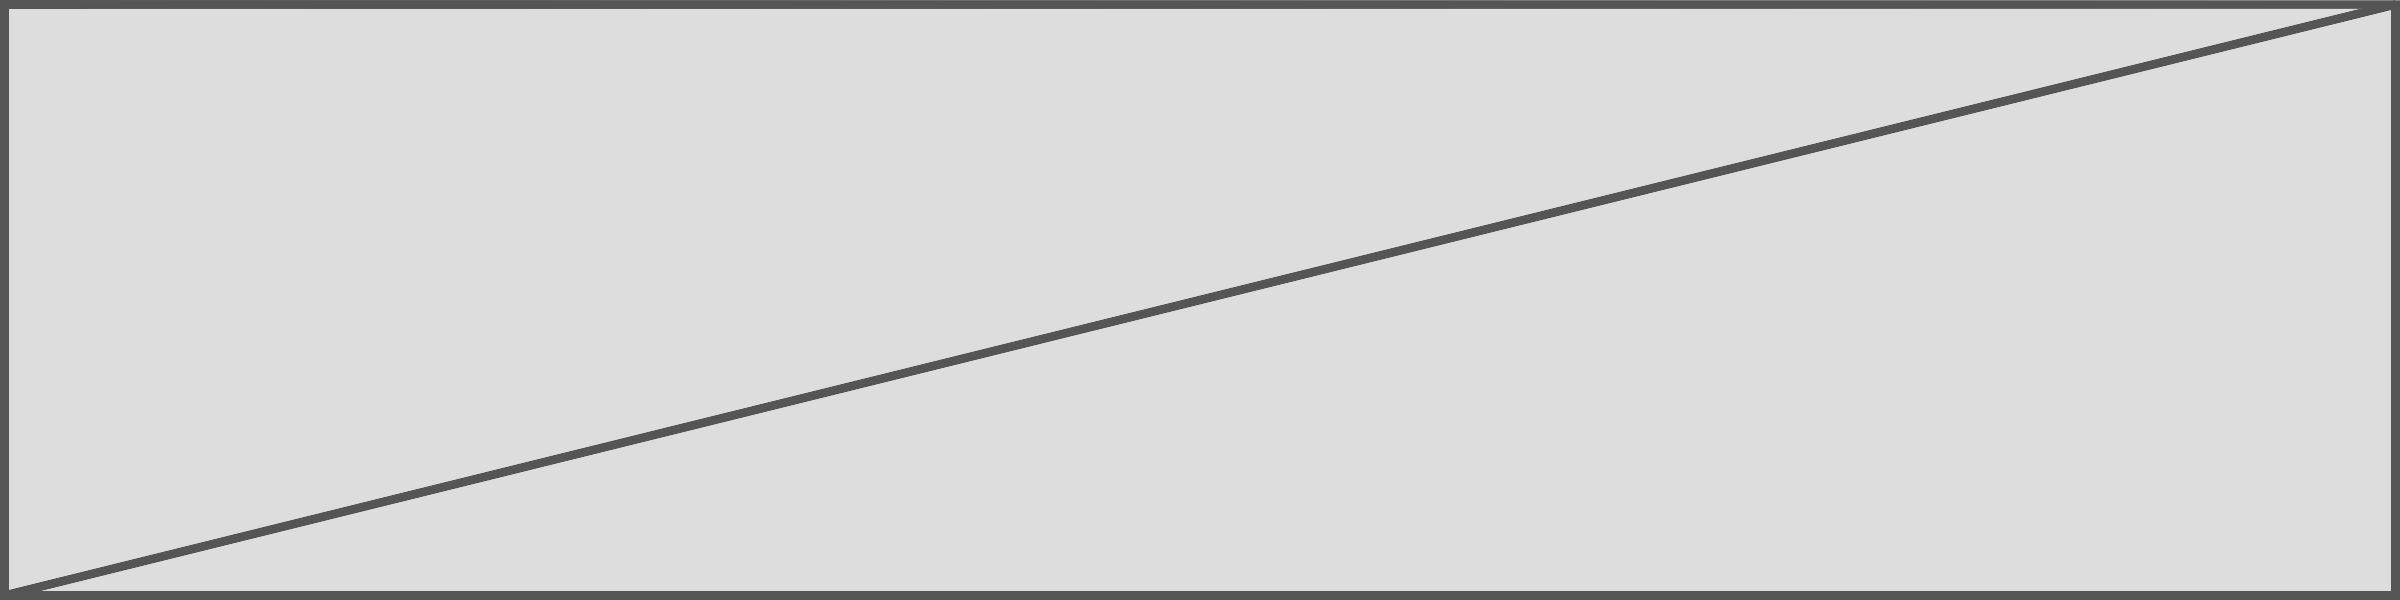
\includegraphics[width=\textwidth]{wide.png}
\caption{A full-width figure. Its caption is long enough to wrap onto a second line, so it is justified with a ragged last line rather than centred: sed ut perspiciatis unde omnis iste natus error sit voluptatem accusantium doloremque laudantium, totam rem aperiam.}
\label{fig:wide}
\end{figure*}

Sed ut perspiciatis unde omnis iste natus error sit voluptatem accusantium doloremque laudantium, totam rem aperiam, eaque ipsa quae ab illo inventore veritatis et quasi architecto beatae vitae dicta sunt explicabo. Nemo enim ipsam voluptatem quia voluptas sit aspernatur aut odit aut fugit, sed quia consequuntur magni dolores eos qui ratione voluptatem sequi nesciunt.
\begin{table}
\caption{A ruled table.}
\label{tab:ruled}
\begin{ruledtabular}
\begin{tabular}{lcr}
Quantity & Symbol & Value \\
\colrule
Speed of light & $c$ & 299792458 \\
Planck constant & $h$ & 6.626 \\
Elementary charge & $e$ & 1.602 \\
\end{tabular}
\end{ruledtabular}
\end{table}

Neque porro quisquam est, qui dolorem ipsum quia dolor sit amet, consectetur, adipisci velit, sed quia non numquam eius modi tempora incidunt ut labore et dolore magnam aliquam quaerat voluptatem. Ut enim ad minima veniam, quis nostrum exercitationem ullam corporis suscipit laboriosam, nisi ut aliquid ex ea commodi consequatur.

Quis autem vel eum iure reprehenderit qui in ea voluptate velit esse quam nihil molestiae consequatur, vel illum qui dolorem eum fugiat quo voluptas nulla pariatur. At vero eos et accusamus et iusto odio dignissimos ducimus qui blanditiis praesentium voluptatum deleniti atque corrupti quos dolores et quas molestias excepturi sint occaecati cupiditate non provident.
\end{document}
